\section{Úvod}
\label{sec:Introduction}

V dnešní době je standardem používat počítač, telefon, tablet a podobná zařízení. A to jak doma, tak i v práci. Podle českého statistického úřadu používalo v roce 2019 více než 80~\% Čechů nad 16 let internet (chytrý telefon~70 \% Čechů) \cite{csu_internet_cesi}. 

S narůstajícím počtem uživatelů internetu roste i množství potenciálních zranitelných cílů. Zároveň pro laiky může být těžké si tuto zranitelnost uvědomovat a to i přes to, že z médií jsou konfrontováni s útoky na společnosti jako je například OKD \cite{okd_hacknuto} nebo nemocnice \cite{nemocnice_hacknuto}. Podle ČSÚ pak byly v roce 2018 napadeny až dvě pětiny velkých firem \cite{csu_hacknuto_podniky}.

Navíc v aktuální situaci koronavirové pandemie, kdy lidé, kteří mohou, pracují převážně z~domova, může narůstat bezpečnostní riziko jejich zaměstnavatelů, protože je komplikovanější zajistit zabezpečení na stejné úrovni jako v interní síti. Také je možné očekávat, že i v budoucnu bude více využívána práce z domova a to jak v zaměstnání, tak i při studiu a to i na nižších stupních vzdělání, kde to donedávna nebylo pravidlem.

Zmíněna rizika mohou být například: %únik citlivých informací, ztráta dat, odepření přístupu, zneužití výpočetního výkonu, krádež identity, stalking .

\begin{itemize}
    \item únik citlivých informací způsobený phishingovým útokem, což je útok často šířený pomocí důvěryhodně vypadající emailové nebo instantní komunikace s cílem získat citlivá data jako přístupové údaje, nebo rootkitem, jenž je škodlivý kód (neboli malware) sloužící útočníkovi, ke vzdálenému přístupu, sběru informací případně modifikaci systémové konfigurace;
    
    \item ztráta dat nebo odepření přístupu, které mohou být způsobeny ransomwarem, což je druh malwaru šifrujícího či mazajícího data;
    
    \item zneužití výpočetního výkonu uživatele botem (opět druh malwaru), a to za účelem těžby kryptoměn nebo zapojení do počítačové sítě zvané botnet, kde každý účastník vykonává požadované operace na základě instrukcí získaných od záškodníka; %BOT
    
    \item krádež identity nebo stalking pomocí škodlivého kódu nazývaného spyware, který útočník využívá k nepozorovanému sledování a sběru informací o oběti \cite{cyberrisks}.
\end{itemize}

Je velmi důležité tyto hrozby včas detekovat a předejít tak ekonomickým a dalším možným dopadům. 

Phishingovým útokům lze do jisté míry předcházet správně nakonfigurovaným obranným softwarem, jenž se snaží komunikaci klasifikovat a~ odhalit tak tento útok. I přesto se však stále útočníkům daří takové útoky realizovat a získat tak od obětí citlivé informace nebo peníze, jak~je~možné ukázat na příkladu nemocnice v Sušici \cite{nemocnice_phishing}. Proto je důležité dostatečně proškolit jedince, kteří mohou být potencionálně zranitelní \cite{antiphishing_solution}.


O detekci škodlivého kódu se snaží především antivirové společnosti, které vyvíjí produkty pro identifikaci přítomnosti malwaru na základě skenování. Škodlivý kód neboli malware je~druh počítačového programu, jehož záměrem je způsobit újmu. Příkladem mohou být jak výše zmíněné ransomwere, spyware nebo rootkit a dále také virus, trojský kůň nebo červ \cite{1425057}. 



%(phishing, keylogger, jež slouží k zaznámení stisku klávesnice), ztráta dat (ransomware je druh kódu, který způsobuje zašifrování nebo odepření přístupu či celkovou ztrátu dat), 

%https://www.icaew.com/-/media/corporate/files/technical/business-and-financial-management/smes/bas-files/top-five-cyber-risks.ashx?la=en

%% https://www.av-test.org/en/statistics/malware/
%% https://interactive.symantec.com/istr24
%% https://docs.broadcom.com/doc/istr-23-2018-en
%% https://resources.malwarebytes.com/files/2020/02/2020_State-of-Malware-Report.pdf

\section{Motivace}

Vzhledem k výše zmíněné závažnosti rizik je potřeba reagovat a odhalit nový malware včas, neboť malware už při prvním kontaktu s obětí může způsobit škodu.

Jak je vidět v grafu (viz obrázek č. \ref{fig:MalwareSamplesAV}) na následujícím obrázku, množství nového malwaru od roku 2011 rostlo zhruba dvojnásobně, nejvíce nového malwaru pak bylo v roce 2015, kdy se~růst počtu nových vzorků prozatím zastavil, nicméně i přesto je jich ročně stále více než 100~milionů.

\begin{figure}[!ht]
    \noindent
    \centering
    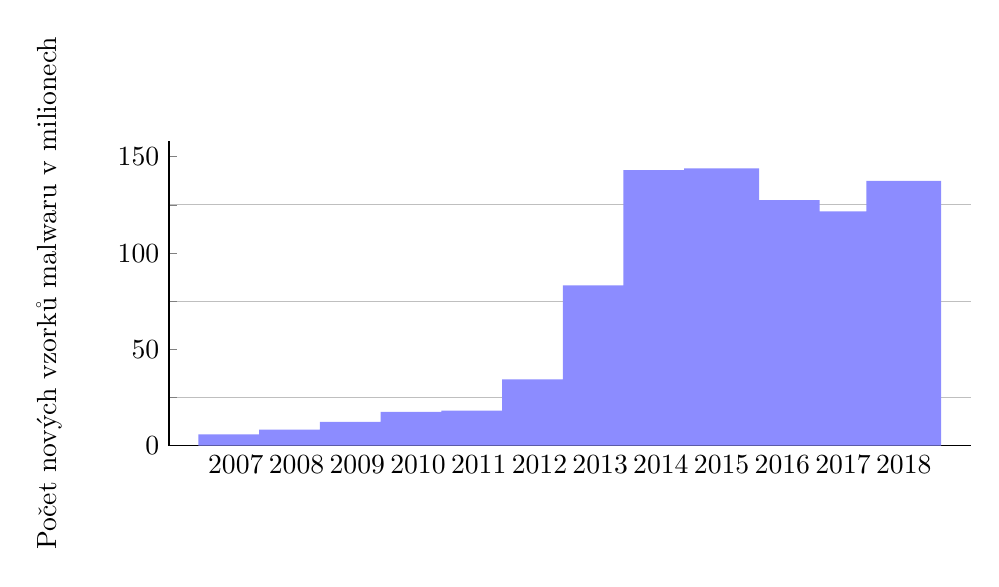
\begin{tikzpicture}
        \begin{axis}[
            ybar,
            bar width=.95cm, 
            width=.97\textwidth,
            height=.45\textwidth,
            ymajorgrids, 
            tick align=inside,
            major grid style={draw=white},
            axis x line*=bottom,
            axis y line*=left,
            ymin = 0,
            yminorgrids = true,
            y axis line style={opacity=100},
            tickwidth=0pt,
            enlarge x limits=true,
            legend style={
                at={(0.5,1)},
                anchor=north,
                /tikz/every even column/.append style={column sep=0.5cm}
            },
            grid=both,
            minor ytick={0, 25,...,150},
            ylabel={Počet nových vzorků malwaru v milionech},
            xtick=data,
            yticklabel style={text width=1cm,align=right},
            /pgf/number format/.cd,
                use comma,
                1000 sep={}
            ]
            nodes near coords={
                %\pgfmathprintnumber[precision=0]{\pgfplotspointmeta}
            }
        ]
        \addplot [draw=none, fill=blue!45] coordinates {
        	    (2007,5.9) 
        	    (2008,8.4)
        		(2009,12.4) 
        		(2010,17.6)
        		(2011,18.2)
        		(2012,34.4)
        		(2013,83.2)
        		(2014,143.1)
        		(2015,144.0)
        		(2016,127.5)
        		(2017,121.7)
        		(2018,137.5)
        	};
        \end{axis}
    \end{tikzpicture}
    
    \caption{Počet vzorků nového malwaru mezi roky 2007 - 2018. Zdroj dat \cite{av_securityreport_1819}}
    \label{fig:MalwareSamplesAV}
    
\end{figure}

Proto jsou vyvíjeny metody automatické analýzy (např. pomocí klasifikace výstupu analýzy kódu a jeho chování viz kapitola \ref{stateOfArt}), jež umožňují získat potřebná data o testovaných vzorcích včas a zmírnit tak případné dopady dosud neodhalené hrozby. Zároveň je také důležité, aby~daný poskytovatel anti-malwarových služeb měl zajištěn dostatečný přísun vzorků, které tvoří reprezentativní zástupce. Takto získané vzorky mohou tvořit databázi malwaru.

%Pro zajištění spolehlivosti testů jsou navrhovány ??
%Dále je také nezbytná spolehlivost analýzy. Proto jsou navrhovány nové postupy

Aby byl zohledněn vznik množství nových vzorků malwaru a také patřičná rychlost analýzy, je navrhováno množství nových přístupů a postupů při odhalování. 

U těchto postupů pak obecně rozlišujeme statickou a dynamickou analýzu, které jsou dále podrobně popsány v teoretické části.

Tato práce se bude dále zabývat především statickou analýzou, možnostmi jejího využití a~to~i~v~kombinaci s dalšími metodami, a jejími limity.

%nevýhody dynamické analýzy: potřeba virtuálního prostředí, které musí odpovídat reálnému (stejná verze operačního systému), 
%výhody statické analýzy: bez potřeby virtuálního prostředí, 

%% State of art
% 7 ruční analýza (popsané programy atd)
% 5 způsob převedení malwaru na obrazek a klasifikace
% 4 limity statické analzy
% 3 android malware analyza
% 2 klasifikace
% 1 staticka a dynamicka
%